\documentclass{beamer}
\usetheme{default}
\begin{document}

\begin{frame}{}

\title{\textbf{Image Processing}}
\maketitle

Chloe Eghtebas, Luke Metz, Brendan Ritter

\end{frame}


\begin{frame}{Basics of Image Processing}

Using computational software to manipulate an image using signal processing techniques.

\end{frame}



\begin{frame}{What You'll Need to Know}

\begin{itemize}
	\item SVD
	\item Convolution
	\item Gaussian blur
\end{itemize}
\end{frame}

\begin{frame}{Image Representation and Software}
Images have 3 channels. Red, Blue, Green. To manipulate these arrays we chose to not use matlab. We chose to use Python and Numpy mainly for its re usability.
\end{frame} 


\begin{frame}{Flipping}

\end{frame}


\begin{frame}{Transformations}

\end{frame}

\begin{frame}{Convolution}
'Blending' two functions together. For discrete data, its like overlapping.
One has original data and a kernel which represents the other function. 
\begin{figure}[htp]
\centering
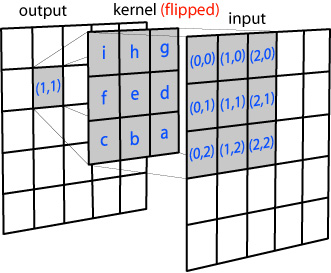
\includegraphics[width=2in]{conv2d_matrix.jpg}
\caption{Convolution in 2D.}
\label{}
\end{figure}
\end{frame}

\begin{frame}{Gaussian Blur}
Application of 

\end{frame}

\begin{frame}{Sobel Edge Detection}

\end {frame}

\begin{frame}{Blur + Edge Detection}

\end{frame}


\begin{frame}{Color}

\end{frame}

\end{document}